\documentclass{article}
\usepackage{epigraph}
\usepackage{graphicx}
\graphicspath{ {./images/} }
\title{6.033 Lecture 1 \\ Operating Systems Part I}
\author{Americo De Filippo}
\begin{document}
\maketitle
\begin{thebibliography}{9}
  \bibitem{texbook}
  Saltzer, Jerome H. and M. Frans Kaashoek. Principles of Computer System Design: An Introduction (2009): \textbf{Sections: 1.1-1.4 and 4.1-4.3.}
\end{thebibliography}
\tableofcontents
\section{Introduction to Systems}
  \epigraph{Everything should be made as simple as possible, but no simpler.}{\textit{Albert Einstein}}
  Much wisdom about systems that has accumulated over the centuries is passed along 
  in the form of folklore, maxims, aphorisms and quotations. Some of that wisdom is 
  captured in the boxes at the bottom of these pages.
  \subsection{Common problems of system in many fields}
    \epigraph{Seek simplicity and distrust it}{\textit{Alfred North Whitehead}}
    The problems that one could encounter when using a system are: emergent properties, propagation of effects, incommensurate scaling and 
    trade-offs. 
  \subsubsection{Emergent Properties}
    \epigraph{Some things turn up only when a thing is built.}{\textit{Unknown}}
    The emergent properties are those that cannot be noticed when designing the singles part of a system, often when a system in built comes 
    up of this emergent properties that we usually call surprise. Sometimes this can be predicted by looking at the system and making 
    some assumptions, like: if I have a fragile roof and I live inside high raining zone, an emergent proprieties could be that 
    my roof will fall when a lot a water will agglomerate on it. But in a lot of times the following rule applies: "\emph{some things turn up only when a thing is built.}"
  \subsubsection{Propagation Effects}
    \epigraph{Our life is frittered away by details... Simplicity, simplicity, simplicity!}{\textit{Henry David Thoreau}}
    A propagation effect is caused when a failure impacts a lot of others parts of the system, when building a system we have to limit the impact 
    on the whole system due to single failure of some part of it. If a part of the system impact too much on the system as a whole we cannot control 
    anymore what a failure in $\alpha$ will cause on the integrity of the whole.
  \subsubsection{Incommensurate Scaling}
    \epigraph{By undue profundity we perplex and enfeeble thought.}{\textit{Edgar Allan Poe}}
    When something is scaled to larger dimensions, it must be done very carefully, when something appear to scale up some of its parts could not do as well,
    for example if a mouse would have the size of an elephant it will collapse due to its skeleton constitution. Hence, when we want to scale up something we 
    must acknowledge that some part of it may not scale as well and for this reason we have to understand that the probability of errors will be 
    increase, and will emerge some others properties as we have known from the first subsection.
  \subsubsection{Trade-offs}
    \epigraph{Fools ignore complexity. Pragmatists suffer it. Some can avoid it. Geniuses remove it}{\textit{Alan J. Perlis}}
    One of the most known issue when creating a system is make good and helpful trade-offs. One form of trade off happens in 'binary classification', this
    form of trade off happens when we want to classify something into two categories in function of the presence or onto the absence of some kind of property 
    In this case we use some indirect measure called \textbf{proxy}. By adjusting the parameters of the proxy a designer is able to reduce one class
    of mistakes. The key is to not look at \textit{ad hoc} examples but rather synthesizing. So, in place of a well-organized theory, we use case studies. For each subtopic 
    in this book, we shall begin by identifying requirements with the apparent intent 
    of deriving the system structure from the requirements. Then, almost immediately 
    we switch to case studies and work backwards to see how real, in-the-field systems 
    meet the requirements that we have set.
  \subsubsection{Systems, Components, interfaces, and environments}
    \epigraph{And simplicity is the unavoidable price we must pay for reliability.}{\textit{Charles Anthony Richard Hoare}}
    Webster’s Third New International Dictionary, Unabridged, defines a system as “a complex 
    unity formed of many often diverse parts subject to a common plan or serving a common purpose.”
    We identify the “many often diverse parts” 
    by naming them components. We identify the “unity” and “common plan” with the inter
    connections of the components, and we perceive the “common purpose” of a system to 
    be to exhibit a certain behavior across its interface to an environment. Thus we formulate 
    our technical definition: a system is a set of interconnected components that 
    has an expected behavior observed at the interface with its environment. \textbf{A system is a set of interconnected components that 
    has an expected behavior observed at the interface with its environment.} 
    When defining a system we have to understand that as in life it's could look different in function of the point of view 
    that we look at it or for the purpose that we are looking for. For example when taking as an example a car, the first point of view could be that of a outside
    viewer. From him point of view the system is characterized from the outside color, from the car's wheels. Whether perhaps
    from the point of view of a passenger, the system is made of the inside components of the car, or the things like the wheels 
    that for the other were a \textbf{component}, for him are just a source of \textbf{noise}. 
  \subsubsection{Complexity}
    \epigraph{It is as if perfection be attained not when there is nothing
      more to add, but when there is nothing more to take away.}{\textit{Antoine de Saint-Exupéry}}
    Webster’s definition of “system” used the word “complex”. Looking up that term, we 
    find that complex means “difficult to understand”. Lack of systematic understanding 
    is the underlying feature of complexity. It follows that complexity is both a subjective 
    and a relative concept. We can hope for defining some underline complexity by identifying 
    some of its core components.
    \begin{enumerate}
      \item \textbf{Large number of components}. Sheer size certainly affects our view of 
        whether a system rates the description “complex”.
      \item \textbf{Large number of interconnections.} Even a few components may be interconnected 
        in an unmanageably large number of ways
      \item \textbf{Many irregularities.} By themselves, many components and interconnections may still represent a 
          simple system, if the components are repetitive and the interconnections are regular
          Even a few components may be interconnected in an unmanageably large number of ways
      \item \textbf{Long Descriptions. }Looking at the best available description of the system 
          one finds that it consists of a long laundry list of properties rather than a short, 
          systematic specification that explains every aspect. Theoreticians formalize this 
          idea by measuring what they call the “Kolmogorov complexity” of a computational 
          object as the length of its shortest specification.
      \item \textbf{A team of designers, implementers, or maintainers. } If a single person is not
          cable of understand a system (from a high level) by himself and is needed a team for arriving
          an understanding, the system is complex.
    \end{enumerate}
  \subsection{The Source of Complexity}
    There are two main sources for complexity in a system, the first is: the number of requirement, and the 
    second is: maintaining high utilization.
    \subsubsection{Cascading and interacting requirements}
      \epigraph{The best is enemy of the good}{\textit{Voltaire}}
      Complexity is a subjective parameter of course, but we can identify some good and reliable characteristic for 
      understand this very important and fundamental part of a software design. A good thing to look at when want to 
      analyze the complexity of a system is the number of requirement of the system. Usually when our system have a 
      lot of requirements to satisfy it will be very complex. The curve that explain this concept better is the following: 
      \begin{figure}[h]
        \centering
        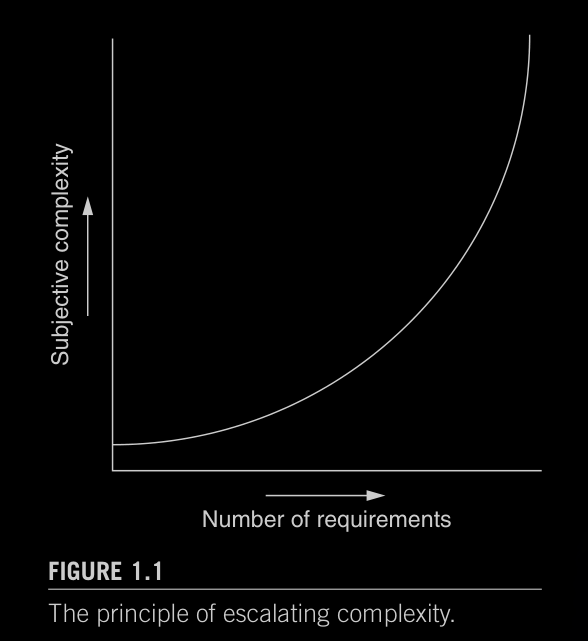
\includegraphics[width=0.50\textwidth]{requirements-graph}
        \caption{}
        \label{fig:mesh1}
      \end{figure}
      \paragraph{The other thing: Generality}
        \epigraph{A complex system that works is invariably found to have evolved from a simple system 
          that works.}{\textit{John Gall}}
        When writing a program we tend to make as general as possible, also when is not needed, because why not? It could need.
        This way of thinking is not always good and efficient especially for a long software that could have a long life. Take for
        example the configuration of a UNIX system like Arch Linux, arch is a good and loved distro cause is amazing customizable and 
        consequentially is incredibly general out of the box. But have you ever tried to use a configuration of another person that perhaps
        has really different taste from yours? It becomes a nightmare, I think you'd be great if you happened to open the terminal. So 
        when designing a system remember to do be careful at the generality that you are aim at, because (if you think about it) at 
        the end of the day simplicity always win. 
    \subsubsection{Maintaining High utilization}
      \epigraph{It is impossible to foresee the consequences of being clever.}{\textit{Christopher Strachey}}
      When we want to have a high efficient application, we could encounter the difficulties
      that these things will imply. Usually when being clever about increase the efficiency of
      a system we are at the same time complicating it. A good picture that summers the concept
      is the following: 
      \begin{figure}[h]
        \centering
        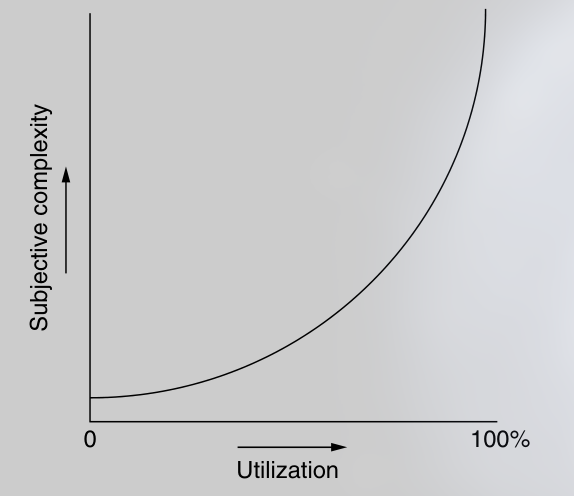
\includegraphics[width=0.50\textwidth]{utilization-graph}
        \caption{}
        \label{fig:mesh2}
      \end{figure}
  \subsection{Coping with complexity I}
  There are some way for handle complexity inside a system, in the next 4 sub section we will
  see 4 of them: modularity, abstraction, layering, and hierarchy
  \subsubsection{Modularity}
    Have you ever tried to compile more than 100 line of code in one time, without 
    any checking when writing. You should try and see how many (silly and not) errors will 
    occur. In general when we write or more generally we organize a thing as an whole big block
    we usually run in a lot of problems. One reason for that could be that we are humans, and 
    we are not able to handle a large amount of information at time. We are better at quality 
    than quantity. The solution in this situation is often to split the system into modules, 
    that we can understand. One of the great power of modularity is also the flexibility of
    changing a single implementation without compromise the entire system (or multiple part
    of it).
  \subsubsection{Abstraction}
    \epigraph{The purpose of computing is insight, not numbers.}{\textit{Richard W. Hamming}}
    For abstraction we basically mean the separation of declaration and implementation, 
    the most common example could be the object-oriented programming that make of the 
    abstraction one of his mainly benefit, or much more in general when we are buying let's
    say a car. We don't want to see all the mechanism inside the engine, but instead we want 
    just to know the horsepower or the 0 to 60 time rate. If there weren't abstraction we
    wouldn't be able to use most of the thing that we use with confident every day.
  \subsubsection{Layering}
    \epigraph{There is no such thing as a small change to a large system.}{\textit{Unknown}}
    This has a lot to do with the first one, let's say that we have our system divided into 
    modules (as the first section taught us), but these modules interact with each other a lot,
    making the system really complex anyway, 'cause we cannot predict the possible change that 
    open module may cause in some other(s). For this reason we want to adopt another principle 
    called layering. The basic rule is this: \textbf{every module in one layer can interact only
    with modules in the same layer.} This may seem a simple rule but is not the case, because 
    creating such structure enables us to have a much more compact and easy debuggable system.
    We see this every day around us take algebra for example:  integers, rationals, complex numbers, 
    polynomials, and polynomials with polynomial coefficients. Each Higher layer communicates with
    a lower one with some simple output.
  \subsubsection{Hierarchy}
    This last principle is something that we are familiar with, all of us have heard of the 
    hierarchy of a company example. This analogy could be very useful cause has a lot of the 
    things that we are interested with. For existing a hierarchy there must be some layering, 
    for being some layering there must be some modularity. But all fits together when 
    hierarchy comes along. In a company the commander of a layer is usually called 'manager', 
    its job is to communicate with the other managers of others layer, in this way him compute
    the information relative to its layer and make the tree (hierarchy) communicate with each other
    reducing the enormous amount of noise that there will be otherwise (if everyone communicates with
    every one).
  \subsubsection{Putting all together: \textit{binding}} 
    One of the most common practice when designing a system is to delay the implementation of 
    the single part of it, instead of implementing we are just giving name to them so that 
    when the system is theorizing we can choose the 'best' implementation for the current
    requirement of the layer. This practice is called: \textit{delay binding}. This is really 
    useful when building a system, 'cause it often happens that we write or think of a particular
    implementation based on the current and most obvious usage of that module, obvious with this 
    technique we can think more through about the implication of that specific module. We can 
    be aware of that by fake the calling of that module when needed, in this way we can test
    the needing empirically.
\section{Enforcing modularity with client and services}
  What we mean for \textbf{enforcing modularity}? \\ As we have said before modularity 
  helps us to have a system divided into sections that we later called layers. But
  there are some problems with this definition, modularity becomes very useful when
  is careful checked by the designer. Because his purpose could be very easily lost
  if a lot of modules communicate with each other in a non-trackable manner. So for 
  \textit{enforcing modularity} we mean to build a system which is capable to track the
  interaction between the modules and in this way enables of us to understand the system 
  (and the errors in it). One way of designing a good enforced modularity is design it 
  as the client and server model, so that the interaction are 'manage' by the tracking 
  of the \textit{messages}, that resemble the only kind of interaction between two or 
  more modules.
  \subsection{From soft to strong modularity}
    When we are dealing with modularity we must be really careful, a good example that will
    justify our shrewdness is the following: \\ suppose that you have two functions: one that 
    calls the other. One of the most common problem that could occur is an error in the callee 
    that will block the caller from its execution. Another common error is the modification of some
    variables passed as parameter that will cause some undefined behavior in the caller and in the
    latter. In these cases our modularity will be defined as \textit{soft}, because it will not 
    check and make sure that there are no side effect in the interaction between the modules, 
    that we have introduced in the first place just for this reason, checking interaction 
    between parts of the system, limiting undefined behaviors. Now we are going to 
    see how we can make this thing work by going from soft to \textit{strong} modularity.
  \subsection{The Client/Service organization} 
    The Client and Service organization is based on a word \textbf{messages}, this word is
    really important for the good working of this organization. The way that this works is 
    not that hard to understand, the modularity strong is based limiting the interaction
    between the modules, making them communicating only via messages that are carefully
    checked by the designer. We have made the distinction between the client and the services
    as we can represent the two part acting in this model. In the previous subchapter we 
    have called the two actors caller and callee, this time we have adopted a new notation
    which is Client (the one who makes the requests) and Services (the one that try to satisfy it).
    The good of this system is that the two of them interact only via messages that are not blocking
    for the most part, and furthermore we could have some kind of checking for the behavior of the 
    Services. Another benefit of this method is the independence that the two of them have, 
    in theory the client is completely independent of the Service, as well as the latter.
 \end{document}
